\scanpage{258}
U N I V E R S I T E\\
DES SCIENCES ET TECHNIQUES\\
\uline{DU LANGUEDOC}\\
AMC/MD

Montpellier, le 24 juin 1975

\uline{Diffusion} : Liste A\\
n\textsuperscript{o} 4135

AVIS DE SOUTENANCE D'UNE THESE DE DOCTORAT DE

\uline{SPECIALITE : CHIMIE}

Mention Chimie Organique Physique

\uline{Nom et prénom du candidat} : DALVERNY Gilbert

\uline{Titre de la thèse} : Synthèse et réactivité d'organomagnésiens perfluorés.
Application à la préparation d'acides perfluorosulfoniques et carboxyliques.

\uline{Date, heure et lieu de soutenance prévus} : 10 juillet 1975 à 11 heures, salle
de cours n\textsuperscript{o} 9 - U.S.T.L.

\uline{Nom du Directeur de thèse} : Monsieur le Professeur A. COMMEYRAS

\uline{Désignation du laboratoire où la thèse est préparée} : Laboratoire de chimie organique

\uline{Analyse de l'ouvrage} : Des méthodes de synthèses, par voie chimique, d'acides
perfluoroalcanesulfoniques \(\mathrm{R_FSO_3H}\) et carboxyliques \(\mathrm{R_FCO_2H}\)
ont été mises au point ; elles font intervenir comme intermédiaires réactionnels, les
organomagnésiens perfluorés saturés \(\mathrm{R_FMgX}\) correspondants.\\
Des possibilités d'application de la réaction magnésienne au niveau de composés
perfluorés insaturés ont été ensuite étudiées.

\uline{Durée approximative des recherches ayant abouti à la thèse} : 2 ans

\uline{Composition du jury proposé} : M. A. COMMEYRAS - Président\\
M. R. CORRIU\\
M. A. CAMBON\\
M. R. MARTIN

Le Secrétaire Général,
\figure{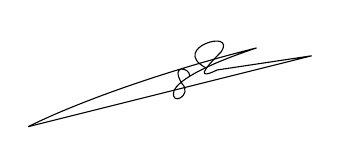
\begin{tikzpicture}[x=1cm,y=1cm]
\draw (0,0) .. controls (.6,.3) and (1.7,.7) .. (2.9,1)
 .. controls (2.3,.8) and (1.9,.6) .. (1.85,.45)
 .. controls (1.8,.25) and (2.1,.4) .. (1.95,.55)
 .. controls (1.8,.8) and (2.05,.75) .. (2.05,.65);
\draw (2.25,.75) .. controls (1.8,1) and (2.65,1.25) .. (2.45,.95)
 .. controls (2.2,.7) and (2.15,.6) .. (2.4,.72)
 --(3.6,.9)--(0,0);
\end{tikzpicture}}
\uline{E. SIAU}
\margin{257}
